\section{Algorithme d'affectation}
\label{sec::moulinette}

\begin{figure}[H]
	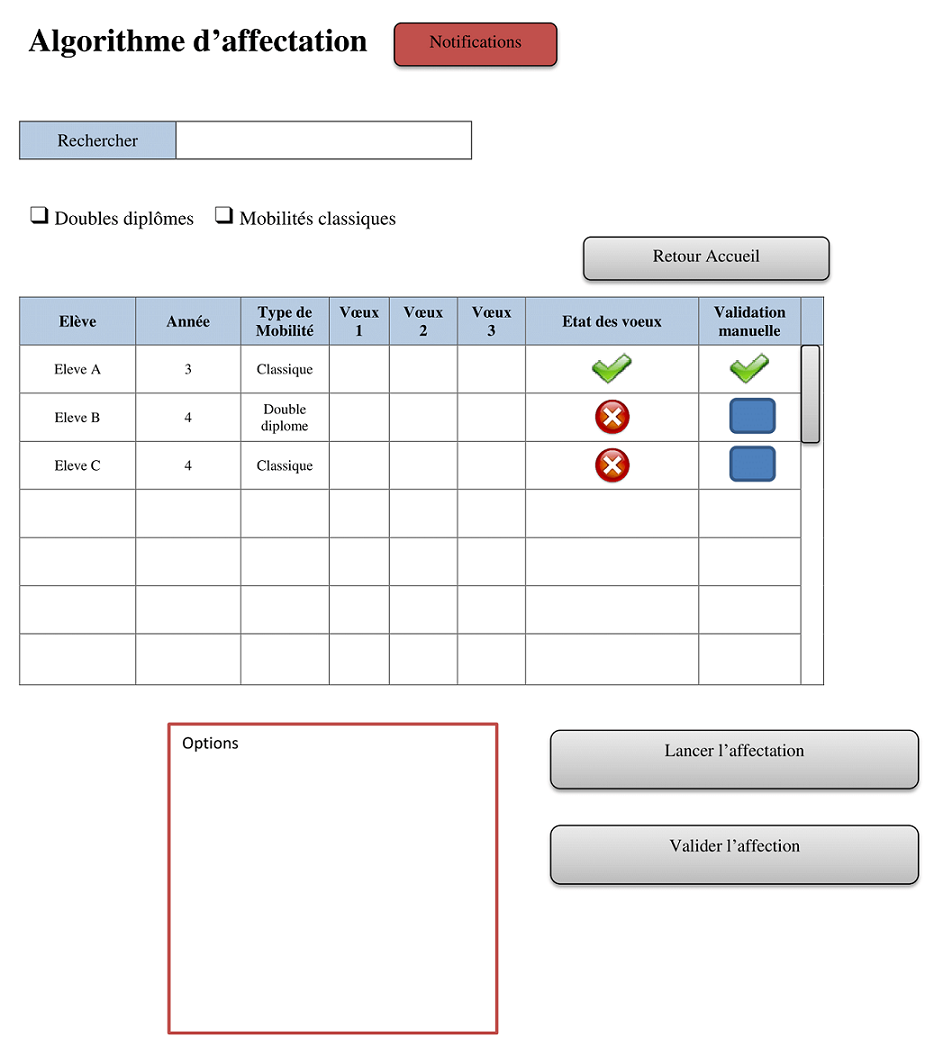
\includegraphics[scale=0.7]{Admin/Moul.png}
	\caption{Page de gestion de l'algorithme d'affectation}
\end{figure}

Sur cette page ce trouve un tableau récapitulant les vœux définitifs des élèves après la fin des choix de vœux (phase 1). Ce tableau comprend donc la liste des élèves, leur année, la liste des vœux, le type de mobilité choisie (double diplôme, mobilité classique), leur état (validé, à validé).

Encore présent sur ce tableau; une zone de recherche par mot clé ainsi que plusieurs filtres (années, universités, type de mobilité...).

\bigbreak

L'administrateur peut, sur cette page, gérer les paramètres de l'algorithme avant de le lancer (ajout de paramètres particuliers modifiant l'ordre d'attribution des vœux, en plus des notes).

\bigbreak

Il est aussi possible à l'administrateur de valider les vœux d'un élève manuellement. Cela fait sortir cet élève de la liste des élèves concernés par l'algorithme (il apparaitra toujours dans la liste des élèves mais son état deviendra "validé" et il ne sera pas pris en compte par l'algorithme).

\bigbreak

Enfin, un bouton permettant de lancer l'algorithme d'attribution des vœux. Lorsque l'algorithme est terminé, la phase 1 est finie et la phase 2 est lancée. Cela signifie que les différentes vues deviendrons celles de la phase 2.